%MIT License
%Copyright (c) 2019 Michele Maione, mikymaione@hotmail.it
%Permission is hereby granted, free of charge, to any person obtaining a copy of this software and associated documentation files (the "Software"), to deal in the Software without restriction, including without limitation the rights to use, copy, modify, merge, publish, distribute, sublicense, and/or sell copies of the Software, and to permit persons to whom the Software is furnished to do so, subject to the following conditions: The above copyright notice and this permission notice shall be included in all copies or substantial portions of the Software.
%THE SOFTWARE IS PROVIDED "AS IS", WITHOUT WARRANTY OF ANY KIND, EXPRESS OR IMPLIED, INCLUDING BUT NOT LIMITED TO THE WARRANTIES OF MERCHANTABILITY, FITNESS FOR A PARTICULAR PURPOSE AND NONINFRINGEMENT. IN NO EVENT SHALL THE AUTHORS OR COPYRIGHT HOLDERS BE LIABLE FOR ANY CLAIM, DAMAGES OR OTHER LIABILITY, WHETHER IN AN ACTION OF CONTRACT, TORT OR OTHERWISE, ARISING FROM, OUT OF OR IN CONNECTION WITH THE SOFTWARE OR THE USE OR OTHER DEALINGS IN THE SOFTWARE.

%INDEX:
%  ABSTRACT
%1 Introduzione
%2 Analisi dello stato dell'arte
%3 Modello teorico
%4 Simulazione e esperimenti
%5 Risultati ottenuti
%6 Commenti conclusivi
%  APPENDIX

\documentclass[journal,A4paper,compsoc,epsfig]{IEEEtran}

\usepackage[cmex10]{amsmath}
\usepackage{amssymb, amsbsy,bm}
\usepackage[noend]{algpseudocode}
\usepackage{algorithm}
\usepackage{array}
\usepackage[italian]{babel}
\usepackage{cite}
\usepackage{graphicx}
\usepackage{listings}
\usepackage[section]{placeins}
\usepackage{stfloats}
\usepackage{url}

\begin{document}
  \title{Implementazione in Python di "Spatial Subspace Rotation"}
  \author{Michele Maione \thanks{Michele Maione - 931468 - michele.maione@studenti.unimi.it, Interazione naturale e Metodi di computazione affettiva, A/A 2018-2019, Universitá degli Studi di Milano, via Celoria 18, Milano, Italia.}}
  \markboth{Implementazione in Python di "Spatial Subspace Rotation", M. Maione}
  {Shell}
  \maketitle

  %ABSTRACT
  \begin{abstract}
    In "A Novel Algorithm for Remote Photoplethysmography - Spatial Subspace Rotation" a cura di W. Wang, S. Stuijk e G. de Haan \cite{wang-tbe-2016}, gli autori propongono un algoritmo (2SR) per la fotopletismografia remota (rPPG).
    
    L'algoritmo 2SR richiede il riconoscimento degli skin-pixels, e per lo scopo è stato utilizzato l'algoritmo (SkinColorFilter) proposto in "Adaptive skin segmentation via feature-based face detection" a cura di M.J. Taylor e T. Morris \cite{adaptive_skin_segmentation}.
    
    L'algoritmo SkinColorFilter riceve in ingresso un volto che deve essere estratto da un filmato.
    L'estrazione del volto è stata ottenuta mediante il classificatore a cascata Haar proposto da P. Viola e M. Jones in "Rapid Object Detection using a Boosted Cascade of Simple Features" \cite{skin_color_filter}.
    
    Ambedue gli algoritmi sono stati implementati in classi Python: SSR.py, SkinColorFilter.py. Mentre per l'estrazione del volto è stata usata la libreria OpenCV.
  \end{abstract}

  %CAP 1
  \section{Introduzione}
    \label{sec:Introduzione}
    La fotopletismografia remota consente di determinare processi fisiologici, come il flusso sanguigno, senza il contatto con la pelle.
    Utilizzando riprese video del viso si analizzano i cambiamenti nel colore della pelle del soggetto che non sono rilevabili dall'occhio umano.
    
    Questa misurazione remota dei livelli di ossigeno nel sangue fornisce un'alternativa senza contatto alla fotopletismografia convenzionale.
    
    Il sistema nervoso autonomo (ANS) è responsabile dell'attuazione delle interazioni psicosomatiche all'interno del corpo umano.
    Molte malattie legate allo stress sono il risultato della compromissione della funzione corporea regolata dall'ANS.
    Uno dei sistemi fisiologici più sensibili alle influenze regolatorie dell'ANS è il sistema cardiovascolare.

    \emph{Importanza del problema}:
      Tutti gli algoritmi rPPG esistenti sfruttano uno schema spazio-temporale comune per l'estrazione dell'impulso, che può essere generalizzato come "temporal combination of spatial color mean".
      Data una sequenza video contenente un soggetto, consiste di due passaggi:
      \begin{enumerate}
        \item Quantificando spazialmente i valori RGB dei pixel della pelle del soggetto in ogni singolo fotogramma (la media RGB);
        \item Creando temporaneamente tracce RGB su più fotogrammi e combinandoli in un segnale.
      \end{enumerate}
      La differenza fondamentale tra questi algoritmi è rappresentata dai diversi criteri utilizzati per combinare le tracce RGB in un segnale di impulso:
      \begin{itemize}
        \item "Blind Source Separation" (basato su PCA oppure su ICA), che utilizza differenti criteri per separare le tracce temporali RGB in indipendenti segnali per estrarre la pulsazione;
        \item CHROM, che combina linearmente i segnali di crominanza assumendo l'utilizzo di un colore di pelle standardizzato per bilanciare il bianco delle immagini;
        \item PBV, che utilizza la firma dei cambiamenti volumetrici del sangue in diverse lunghezze d'onda, per dinstinguere esplicitamente il cambiamento di colore indotto dalla pulsazione, tramite il rumore nelle misurazioni RGB;
        \item 2SR, che misura la rotazione temporale del sottospazio degli skin-pixels per l'estrazione della pulsazione.
      \end{itemize}
      L'algoritmo 2SR consiste di due passaggi:
      \begin{enumerate}
        \item Nel dominio spaziale, un sottospazio di skin-pixel è costruito nello spazio RGB;
        \item Nel dominio temporale, l'angolo di rotazione dei sottospazi degli skin-pixels tra fotogrammi successivi viene misurato per l'estrazione dell'impulso.
      \end{enumerate}

    \emph{Approccio seguito}:
      L'algoritmo 2SR presuppone l'esistenza di sensori pixel della camera spazialmente ridondanti e una ben definita skin mask.
      
      L'idea di base è di stimare un sottospazio degli skin-pixel e misurare la sua rotazione temporale per l'estrazione della pulsazione, che non richiede a priori la tonalità della pelle o degli impulsi, in contrasto con gli algoritmi esistenti.
      
      L'estrazione del volto dal filmato è stata ottenuta mediante il classificatore a cascata Haar proposto da P. Viola e M. Jones in "Rapid Object Detection using a Boosted Cascade of Simple Features" \cite{skin_color_filter}.
      
      Per il riconoscimento degli skin-pixels è stato utilizzato l'algoritmo SkinColorFilter proposto da M.J. Taylor e T. Morris. in "Adaptive skin segmentation via feature-based face detection" \cite{adaptive_skin_segmentation}.
      
      Ambedue gli algoritmi sono stati implementati in classi Python: SSR.py, SkinColorFilter.py. Mentre per l'estrazione del volto è stata usata la libreria OpenCV.

  %CAP 2
  \section{Analisi dello stato dell'arte}
    \label{sec:Analisi}
    %metodi PCA, ICA: Blind Source Separation
    %metodi CHROM, PBV    
    I metodi remoti esistenti per ottenere la frequenza cardiaca da sequenze video possono essere classificati come: metodi basati sull'intensità del colore e metodi basati sul movimento.
    Attualmente, i metodi basati sull'intensità sono i più popolari.

    \subsection{Metodi basati sull'intensità}
      I metodi basati sull'intensità estraggono i segnali PPG catturati dalle fotocamere digitali.
      Il sangue assorbe la luce più dei tessuti circostanti e le variazioni volumetriche sanguigne influenzano la trasmissione della luce e la riflettanza.
      Ciò porta a sottili cambiamenti di colore sulla pelle umana, che sono invisibili agli occhi umani ma non alle telecamere.
      
      Diversi modelli ottici vengono applicati per estrarre l'intensità dei cambiamenti di colore causati dal battito.
      L'emoglobina e l'ossiemoglobina hanno entrambe: un'elevata capacità di assorbimento nell'intervallo del colore verde e una bassa capacità nell'intervallo del colore rosso.
      Ma tutti e tre i canali di colore contengono informazioni PPG.
      
      Per classificare i metodi esistenti, dividiamo la procedura di rilevamento della frequenza cardiaca in tre fasi: elaborazione del video del volto, estrazione del segnale BVP (Blood Volume Pulse) della faccia e calcolo della frequenza cardiaca.

      \subsubsection{Elaborazione video del volto}
        L'elaborazione video del volto ha lo scopo di rilevare i volti, migliorare la robustezza rispetto al movimento, ridurre gli errori di quantizzazione e preparare i segnali in primo piano per un'ulteriore estrazione del segnale BVP.
        Esistono vari algoritmi per questa fase rispetto a quelle d'estrazione del segnale BVP e del calcolo della frequenza cardiaca.    
        
      \subsubsection{Calcolo della frequenza cardiaca}
        La fase di calcolo della frequenza cardiaca mira a calcolare la frequenza cardiaca dal segnale cardiaco ottenuto nella fase precedente.
        In questa fase, i metodi possono essere raggruppati in analisi del dominio del tempo e analisi del dominio della frequenza:
        \begin{itemize}
          \item Per l'elaborazione nel dominio del tempo, viene applicato diffusamente il rilevamento del picco, per ottenere l'intervallo tra battiti (IBI), da cui viene calcolata la frequenza cardiaca;
          \item Nel dominio della frequenza, viene utilizzata principalmente la densità spettrale di potenza, in cui la frequenza dominante viene presa come frequenza cardiaca. Il calcolo della frequenza cardiaca può diventare complesso per applicazioni che includono funzioni di gestione del buffer per presentare i risultati della frequenza cardiaca dopo un certo periodo di tempo.
        \end{itemize}

    \subsection{Metodi principali}
      \subsubsection{CVPR14 - Remote Heart Rate Measurement From Face Videos Under Realistic Situations \cite{Li:2014}}
        L'algoritmo per recuperare il segnale di impulso può essere suddiviso in diversi passaggi:
        \begin{itemize}
          \item Estrazione di segnali rilevanti dalla sequenza video (vale a dire colore della pelle e colore di sfondo);
          \item Correzione per l'illuminazione globale;
          \item Eliminazione del movimento non rigido;
          \item Filtering.
        \end{itemize}

      \subsubsection{CHROM - Robust Pulse Rate From Chrominance-Based rPPG \cite{deHaan:2013}}
        L'algoritmo per recuperare il segnale di impulso può essere suddiviso in diversi passaggi:
        \begin{itemize}
          \item Estrazione dei segnali del colore della pelle dalla sequenza video;
          \item Proiezione del colore medio della pelle nello spazio, definito, di crominanza;
          \item Filtro passa banda nello spazio di crominanza;
          \item Costruire il segnale della pulsazione.
        \end{itemize}
  
  %CAP 3
  \section{Modello teorico}
    \label{sec:Modello}
    L'idea principale dell'algoritmo è di misurare la rotazione temporale del sottospazio degli skin-pixels per estrarre la pulsazione.
    I due passi da eseguire sono:
    \begin{itemize}
      \item Nel dominio spaziale, un sottospazio di skin-pixels è costruito nello spazio RGB;
      \item Nel dominio temporale, l'angolo di rotazione del sottospazio tra fotogrammi consecutivi è misurato per estrarre la pulsazione.
    \end{itemize}
    
    \subsection{Costruizione del sottospazio di skin-pixels}
      Data la matrice $V_{N \times 3}$, degli $N$ skin-pixels vettorizzata sui canali RGB, allora la matrice simmetrica di correlazione spaziale RGB, $C_{3 \times 3}$, è data da:
      \begin{equation}
        C = \frac{V^{\top} \cdot V}{N}
        \label{eq:SCM}
      \end{equation}
      per ogni matrice simmetrica reale $N \times N$, gli autovalori $\Lambda_{3 \times 3}$ sono reali e gli autovettori $U_{3 \times 3}$ possono essere scelti in modo tale che siano ortogonali tra loro:
      \begin{equation}
        C = U \cdot \Lambda \cdot U^{\top}
        \label{eq:CScomposition2}
      \end{equation}
      per la (\ref{eq:CScomposition2}) possiamo quindi scomporre $C$ in questo modo:
      \begin{equation}
        C =
          \lambda_1 \cdot u_1 \cdot u^{\top}_1 +
          \lambda_2 \cdot u_2 \cdot u^{\top}_2 +
          \lambda_3 \cdot u_3 \cdot u^{\top}_3
        \label{eq:CScomposition3}
      \end{equation}
      per cui il principale autovettore $u_1$ è lo skin-vector dominante nel cluster degli skin-pixels, $u_2$ e $u_3$ sono direzioni di variazione e sono ortogonali a $u_1$.

    \subsection{Misurazione dell'angolo di rotazione del sottospazio tra fotogrammi}
      Nel dominio temporale, la pulsazione sanguigna provoca variazioni nei canali RGB e, quindi, modifica il sottospazio degli skin-pixels.
      Poiché il sottospazio è costruito da skin-pixels spazialmente ridondanti senza normalizzazione temporale, non possiamo usare direttamente la traslazione subspaziale per misurare l'impulso,
      perché le variazioni pulsatili senza normalizzazione temporale sono proporzionali all'intensità della luminanza e, quindi, in una relazione moltiplicativa.
      Modelliamo la relazione temporale tra due sottospazi come rotazione e scalatura istantanea:
      \begin{enumerate}
        \item La rotazione tra autovettori (cambiamento di direzione) è correlata ai diversi contributi PPG nei canali RGB;
        \item Il cambiamento degli autovalori (variazione di energia) è correlato alla pulsatilità della pelle misurata.
      \end{enumerate}
      Poiché il sottospazio $U_{3 \times 3}$ è costituito da autovettori con norma unitaria, i suoi cambiamenti temporali possono solo causare una rotazione.
      Quindi, definiamo un passo temporale con la lunghezza $l$ per analizzare la rotazione subspaziale.
      Considerando il sottospazio nel primo fotogramma di un passo $U_{\tau}$ come riferimento, la rotazione tra $U_{t, t \leq l}$ e $U_{\tau}$ è la matrice di rotazione $R_{3 \times 3}$:
      \begin{equation}
        R = {U_t}^{\top} \cdot U_{\tau} =
        \begin{pmatrix}
          {u^t_1}^{\top} \\
          {u^t_2}^{\top} \\
          {u^t_3}^{\top}
        \end{pmatrix} \cdot
        \begin{pmatrix}
          u^{\tau}_1 &
          u^{\tau}_2 &
          u^{\tau}_3
        \end{pmatrix}.
        \label{eq:RotationMatrix}
      \end{equation}
      Poiché la norma euclidea degli autovettori è normalizzata a $1$, gli elementi in $R$ rappresentano essenzialmente gli angoli del coseno tra autovettori:
      \begin{equation}
        cos(\theta_{i, j}) = \frac{{u^t_i}^{\top} \cdot u^{\tau}_j}{\lVert u^t_i \rVert \cdot \lVert u^{\tau}_j \rVert}.
        \label{eq:CosNorm}
      \end{equation}
      Quindi, $R$ può essere riscritto come:
      \begin{equation}
        R =
        \begin{pmatrix}
          cos(\theta_{11}) && cos(\theta_{12}) && cos(\theta_{13}) \\
          -cos(\theta_{12}) && cos(\theta_{22}) && cos(\theta_{23}) \\
          -cos(\theta_{13}) && -cos(\theta_{23}) && cos(\theta_{33})
        \end{pmatrix}.
        \label{eq:RotationMatrixCos}
      \end{equation}
      A causa dell'ortogonalità degli autovettori in $U$, il coseno nelle voci non diagonali misura effettivamente le variazioni dell'angolo seno.
      Quindi, $R$ può essere riscritto come:
      \begin{equation}
        R =
        \begin{pmatrix}
          cos(\theta_{11}) && sin(\theta_{12}) && sin(\theta_{13}) \\
          -sin(\theta_{12}) && cos(\theta_{22}) && sin(\theta_{23}) \\
          -sin(\theta_{13}) && -sin(\theta_{23}) && cos(\theta_{33})
        \end{pmatrix}.
        \label{eq:RotationMatrixCosSin}
      \end{equation}
      La pulsazione sanguigna cambia il tono della pelle, che è in effetti lo skin-vector dominante $u_1$ nello spazio RGB. Quindi, solo la rotazione temporale di $u_1$ è considerata.
      Tuttavia, come spiegato in precedenza, la rotazione tra $u^t_1$ e $u^{\tau}_1$ non può essere utilizzata.
      Misuriamo solo la rotazione tra il vettore $u^t_1$ e il piano ortonormale come:
      \begin{equation}
        R' =
        \begin{pmatrix}
          {u^t_1}^{\top}
        \end{pmatrix} \cdot
        \begin{pmatrix}        
          u^{\tau}_2 &
          u^{\tau}_3
        \end{pmatrix} =
        \begin{pmatrix}
          {u^t_1}^{\top} \cdot u^{\tau}_2 &
          {u^t_1}^{\top} \cdot u^{\tau}_3
        \end{pmatrix}.
        \label{eq:RRoration}
      \end{equation}
      Oltre alla rotazione subspaziale, anche gli autovalori corrispondenti alla varianza/energia degli autovettori sono influenzati dalla pulsazione sanguigna. Poiché $\lambda_i$, scomposta da $C$, è la potenza della varianza, ne deriviamo le variazioni di scala come:
      \begin{equation}
        S =
        \sqrt{\lambda^t_1} \cdot diag \left(
        \begin{pmatrix}        
          \sqrt{\lambda^{\tau}_2} && 0 \\
          0 && \sqrt{\lambda^{\tau}_3}
        \end{pmatrix}^{-1} \right) =
        \begin{pmatrix}
          \sqrt{\frac{\lambda^{t}_1}{\lambda^{\tau}_2}} \\
          \sqrt{\frac{\lambda^{t}_1}{\lambda^{\tau}_3}}
        \end{pmatrix}.
        \label{eq:SScale}
      \end{equation}
      I segnali prodotti da $S$ rappresentano il cambiamento della scala/energia del sottospazio ruotato, che è in realtà correlato alla pulsatilità della pelle misurata.
      Tuttavia, se i riflessi della pelle contengono anche le variazioni di intensità dello spettro (ad es. causate dal movimento), anche $S$ potrebbe esserne influenzato.
      Quindi, non possiamo solo usare gli autovalori per ricavare l'impulso.
      Poiché $S$ è stimato rispetto al sottospazio di riferimento, possiamo limitare i suoi cambiamenti alla direzione della rotazione subspaziale combinando (\ref{eq:SScale}) con (\ref{eq:RRoration}):
      \begin{equation}
        SR = S^{\top} \odot R'.
        \label{eq:SRScalingRotation}
      \end{equation}      
      Per ottenere un $SR$ coerente nel tempo, $SR$ deve essere analizzato nello stesso spazio. Quindi viene proiettato nello spazio RGB originale, cosicché il problema del segno arbitrario della decomposizione degli autovalori, dopo la retroproiezione è rimosso:
      \begin{equation}
        SR' = SR \cdot
        \begin{pmatrix}
          {u^{\tau}_2}^{\top} \\
          {u^{\tau}_3}^{\top}
        \end{pmatrix}.
        \label{eq:CoherentSR}
      \end{equation}      
      Deriviamo/amplifichiamo il segnale di impulso combinando le prime due tracce anti-fase, $\vec{p}_{l \times 1}$, utilizzando $\vec{SR'_i}$, che è l'i-esima traccia di $SR'$:
      \begin{equation}
        \vec{p} = \vec{SR'_1} - \frac{\sigma(\vec{SR'_1})}{\sigma(\vec{SR'_2})} \cdot \vec{SR'_2}.
        \label{eq:pPulseSignal}
      \end{equation}
      Il segnale di impulso a lungo termine $\vec{P}_{K \times 1}$, viene stimato da passi successivi usando l'aggiunta per sovrapposizione:      
      \begin{equation}
        \vec{P}^{t - l} = \vec{P}^{t - l} + (\vec{p} - \mu(\vec{p})).
        \label{eq:LongTermPulseSignal}
      \end{equation}
      
  %CAP 4
  \section{Simulazione e esperimenti}
    \label{sec:Simulazione}
    Sul dataset COHFACE sono stati eseguiti i test dei 6 algoritmi per la fotopletismografia remota, e sono stati comparati i risultati.

    \subsection{Dataset}
      \label{dataset}
      Il dataset utilizzato è il COHFACE della Idiap Research Institute.
      Esso contiene 160 sequenze video RGB, della durata di 100 secondi, di 40 soggetti (12 femmine e 28 maschi) con 4 differenti livelli di illuminazione e rotazione della testa. Le registrazioni dei volti sono sincronizzate con la frequenza cardiaca e quella respiratoria del soggetto esaminato.
      
      Le sequenze video sono state registrate con un Logitech HD C525 a una risoluzione di 640x480 pixel e un frame rate di 20Hz, mentre i segnali fisiologici sono stati acquisiti utilizzando i dispositivi della Tought Technologies insieme alla suite software BioGraph Infiniti v5.
      
      Nella cartella \path{./samples/} ci sono le 40 cartelle contenenti i video dei soggetti.

    \subsection{Architettura del sistema}
      \label{arch}
      L'algoritmo è stato sviluppato per Python 3.6, utilizzando le seguenti librerie:
      \begin{itemize}
        \item numpy (numpy 1.16, \url{http://www.numpy.org});
        \item cv2 (opencv-python 4.0, \url{http://opencv.org});
        \item skimage (scikit-image 0.14, \url{http://scikit-image.org}).
      \end{itemize}      
      È stato utilizzato un classificatore a cascata Haar, che necessita del file delle definizioni collocato in: \path{./data/haarcascade_frontalface_default.xml}.      
      L'algoritmo può essere eseguito con il comando:
      \begin{lstlisting}[language=bash,breaklines=true]
        python3.6 virtualHeartRate.py $VideoFilePath $Method $RangeInSeconds $StepsInSeconds $OutFilePath $ShowVideo
      \end{lstlisting}
      passando al parametro "Method" il valore 0.
      Un esempio di esecuzione è il seguente:
      \begin{lstlisting}[language=bash,breaklines=true]
        python3.6 virtualHeartRate.py samples/1/1/data.avi 0 10 10 outs/out_1_1.txt 0
      \end{lstlisting}

    \subsection{Dettagli implementativi}
      L'algoritmo utilizzato per la fotopletismografia remota proposto da Wang, Stuijk e de Haan \cite{wang-tbe-2016} è il seguente:
      \begin{algorithm}[!htb]
        \caption{Spatial Subspace Rotation}
        \label{SpatialSubspaceRotation}

        \begin{algorithmic}[1]
          \renewcommand{\algorithmicrequire}{\textbf{Input:}}
          \renewcommand{\algorithmicensure}{\textbf{Output:}}
          
          \Require {a video sequence containing K frames}
          
          \State {$\vec{P} = zeros(1, K)$}

          \For{$k = 1, 2, \dots, K$}
            \State{$C^k = \frac{V^{k\top} \cdot V^k}{N}$}
            
            \State {$[\Lambda^{k}, U^{k}] = eigs(C^k)$}

            \If{$\tau = k - l + 1 > 0$}
              \For{$t = \tau, \tau + 1, \dots, k$}
                \State{$SR' = \sqrt{\frac{\lambda_{0}^{t}}{\lambda_{1}^{\tau}}} \cdot {u_{0}^{t}}^{\top} \cdot u_{1}^{\tau} \cdot {u_{1}^{\tau}}^{\top} + \sqrt{\frac{\lambda_{0}^{t}}{\lambda_{2}^{\tau}}} \cdot {u_{0}^{t}}^{\top} \cdot u_{2}^{\tau} \cdot {u_{2}^{\tau}}^{\top}$}

                \State{$\vec{SR'} \leftarrow$ concatenated by SR'}
              \EndFor

              \State{$\vec{p} = \vec{SR'}_0 - \frac{\sigma(\vec{SR'}_0)}{\sigma(\vec{SR'}_1)} \cdot \vec{SR'}_1$}
              \State{$\vec{P}^{t-l} = \vec{P}^{t-l} + (\vec{p} - \mu(\vec{p}))$}
            \EndIf
          \EndFor

          \Ensure {the pulse-signal $\vec{P}$}          
        \end{algorithmic}
      \end{algorithm}

      \subsubsection{L'algoritmo \ref{calulatePulseSignal} è l'implementazione in Python dell'algoritmo \ref{SpatialSubspaceRotation}. Esso necessita di un algoritmo per l'individuazione del volto in un frame (il classificatore a cascata Haar utilizzando OpenCV) e dell'algoritmo \ref{getSkinPixels} per l'estrazione degli skin-pixels.}
        Gli algoritmi per il calcolo della pulsazione sono stati tratti da \cite{wang-tbe-2016}:
        \begin{itemize}
          \item calulatePulseSignal: Calcola il segnale della pulsazione P;
          \item buildP: Costruisce il segnale p da aggiungere alla pulsazione P;
          \item buildCorrelationMatrix: Costruisce la matrice di correlazione C dalla mappa dalla matrice degli skin-pixels V.
        \end{itemize}
        \noindent
        Per estrarre gli skin-pixels sono stati usati i seguenti algoritmi tratti da \cite{adaptive_skin_segmentation}:
        \begin{itemize}
          \item getSkinPixels: Estrae skin-pixels dai volti;
          \item RGMask: Calcola la maschera Red-Green;
          \item generateCircularMask: Genera la maschera circolare del volto;
          \item removeLuma: Rimuove i pixel con valori di luminanza estremi;
          \item EGP: Stima i parametri gaussiani dall'immagine;
          \item getSkinMask: Ottiene la skin-mask.
        \end{itemize}

        \begin{algorithm}[!htb]
          \caption{Calcola il segnale pulsazione P}
          \label{calulatePulseSignal}

          \begin{algorithmic}[1]
            \Function{calulatePulseSignal}{$images, fps$}
              \State {$l \leftarrow fps$}
              \Comment {passo temporale}
              
              \State {$K \leftarrow images.x$}
              \Comment {numero di frames}

              \State {$P \leftarrow zeros((K))$}
              
              \State {$xml \leftarrow "HaarCascadeFrontalFace.xml"$}
              \State {$HaarCC \leftarrow OpenCV.CascadeClassifier(xml)$}
              
              \For{$k \leftarrow 0$ \textbf{to} $K$}
                \State {$img \leftarrow images[k]$}
                \State {$faces \leftarrow HaarCC.detectMultiScale(img)$}
              
                \If{$len(faces) = 1$}
                  \State {$V \leftarrow getSkinPixels(faces, img, k = 0)$}
                  \State {$C \leftarrow buildCorrelationMatrix(V)$}
                  \Comment {$C_{3 \times 3}$}

                  \State {$\Lambda^{k}, U^{k} \leftarrow eigs(C)$}

                  \If{$k \geq l$}
                    \State {$\tau \leftarrow k - l$}
                    \State {$p \leftarrow buildP(\tau, k, l, U, \Lambda)$}
                    \Comment {$p_{l \times 1}$}

                    \State {$P^{t-l} \leftarrow P^{t-l} + p$}
                  \EndIf
                \EndIf
              \EndFor

              \State{\Return {$P$}}
            \EndFunction
          \end{algorithmic}
        \end{algorithm}
        
        \begin{algorithm}[!htb]
          \caption{Costruisce il segnale p}
          \label{buildP}
          
          \begin{algorithmic}[1]
            \Function{buildP}{$\tau, k, l, U, \Lambda$}
              \State{$SR \leftarrow zeros((3, l))$}
              
              \For{$t \leftarrow \tau$ \textbf{to} $k$}
                \State{$A \leftarrow \sqrt{\frac{\Lambda_{0}^{t}}{\Lambda_{1}^{\tau}}} \cdot {U_{0}^{t}}^{\top} \otimes U_{1}^{\tau} \otimes {U_{1}^{\tau}}^{\top}$}
                \Comment{$A_{3 \times 1}$}

                \State{$B \leftarrow \sqrt{\frac{\Lambda_{0}^{t}}{\Lambda_{2}^{\tau}}} \cdot {U_{0}^{t}}^{\top} \otimes U_{2}^{\tau} \otimes {U_{2}^{\tau}}^{\top}$}
                \Comment{$B_{3 \times 1}$}

                \State{$SR^{t} \leftarrow A + B$}
              \EndFor

              \State{$p \leftarrow SR_0 - \frac{\sigma(SR_0)}{\sigma(SR_1)} \cdot SR_1$}
              \State{$p' \leftarrow \mu(p)$}

              \State{\Return {$p'$}}
              \Comment {$p'_{l \times 1}$}
            \EndFunction
          \end{algorithmic}
        \end{algorithm}
        
        \begin{algorithm}[!htb]
          \caption{Costruisce la matrice di correlazione da V}
          \label{buildCorrelationMatrix}
          
          \begin{algorithmic}[1]
            \Function{buildCorrelationMatrix}{$V$}
              \State{$N \leftarrow V.y$}
              \Comment {numero di skin-pixels}

              \State{$C \leftarrow \frac{V^{\top} \cdot V}{N}$}
              \Comment {$V_{3 \times N}$}
              
              \State{\Return {$C$}}
              \Comment {$C_{3 \times 3}$}
            \EndFunction
          \end{algorithmic}
        \end{algorithm}

        \begin{algorithm}[!htb]
          \caption{Ottiene autovalori e autovettori, ordinali}
          \label{eigs}
          
          \begin{algorithmic}[1]
            \Function{eigs}{$C$}
              \State{$\Lambda, U = eig(C)$}
              \Comment {numpy.linalg.eig}

              \State{$idx = \Lambda.argsort()$}
              \Comment {numpy.argsort}

              \State{$\Lambda' = \Lambda_{idx}$}
              \Comment {ordina autovalori}

              \State{$U' = U_{idx}$}
              \Comment {ordinati in base agli autovalori}
      
              \State{\Return {$\Lambda', U'$}}
              \Comment {$\Lambda'_{3 \times 1}, U'_{3 \times 3}$}
            \EndFunction
          \end{algorithmic}
        \end{algorithm}

        \begin{algorithm}[!htb]
          \caption{Estrae skin-pixels dai volti}
          \label{getSkinPixels}

          \begin{algorithmic}[1]
            \Function{getSkinPixels}{$faces, img, doSkinInit$}
              \For{$(x, y, w, h) \leftarrow faces$}
                \State {$ROI \leftarrow img[y:y + h, x:x + w]$}
                \Comment {$ROI_{w \times h \times 3}$}
              \EndFor

              \If{$doSkinInit$}
                \State {$M, C, CI, MU \leftarrow EGP(ROI)$}
              \EndIf

              \State {$skinMask \leftarrow getSkinMask(ROI, CI, MU, 0.5)$}
              \State {$V \leftarrow ROI[skinMask]$}

              \State{\Return {$V$}}
              \Comment {$V_{w \cdot h \times 3}$}
            \EndFunction
          \end{algorithmic}
        \end{algorithm}

        \begin{algorithm}[!htb]
          \caption{Calcola maschera Red-Green}
          \label{RGMask}

          \begin{algorithmic}[1]
            \Function{RGMask}{$img$}
              \State {$R \leftarrow zeros((img.x, img.y))$}
              \State {$G \leftarrow zeros((img.x, img.y))$}

              \State {$channelSum \leftarrow img_0 + img_1 + img_2$}
              \State {$non0mask \leftarrow img_0 \lor img_1 \lor img_2$}

              \State {$R[non0mask] \leftarrow \frac{img[non0mask, 0]}{channelSum[non0mask]}$}              
              \State {$G[non0mask] \leftarrow \frac{img[non0mask, 1]}{channelSum[non0mask]}$}
              
              \State{\Return {$R, G$}}
              \Comment {$R_{img.x \times img.y}, G_{img.x \times img.y}$}
            \EndFunction
          \end{algorithmic}
        \end{algorithm}
        
        \begin{algorithm}[!htb]
          \caption{Maschera circolare del volto}
          \label{generateCircularMask}
          
          \begin{algorithmic}[1]
            \Function{generateCircularMask}{$img, rRatio$}
              \State{$w \leftarrow img.x$}
              \State{$h \leftarrow img.y$}
      
              \State{$xCenter \leftarrow \frac{w}{2}$}
              \State{$yCenter \leftarrow \frac{h}{2}$}
              
              \State{$X \leftarrow zeros((w, h))$}
              \State{$Y \leftarrow zeros((h, w))$}

              \State{$X_x \leftarrow range(0, w)$}
              \State{$Y_x \leftarrow range(0, h)$}

              \State{$Y \leftarrow Y^{\top}$}
      
              \State{$X \leftarrow X - xCenter$}
              \State{$Y \leftarrow Y - yCenter$}
              \Comment{sposta il centro nell'origine}
    
              \State{$r \leftarrow rRatio \cdot h$}
      
              \State{$cMask \leftarrow X^2 + Y^2 < r^2$}
              \Comment{matrice booleana}

              \State{\Return {$cMask$}}
              \Comment{$cMask_{w \times h}$}
            \EndFunction
          \end{algorithmic}
        \end{algorithm}

        \begin{algorithm}[!htb]
          \caption{Rimozione pixel con valori luma estremi}
          \label{removeLuma}
          
          \begin{algorithmic}[1]
            \Function{removeLuma}{$img, cMask$}
              \State{$R \leftarrow 0.299 \cdot img[cMask, 0]$}
              \State{$G \leftarrow 0.587 \cdot img[cMask, 1]$}
              \State{$B \leftarrow 0.114 \cdot img[cMask, 2]$}
      
              \State{$luma \leftarrow R + G + B$}
      
              \State{$m \leftarrow \mu(luma)$}
              \Comment{$numpy.mean$}
              \State{$s \leftarrow \sigma(luma)$}
              \Comment{$numpy.std$}
      
              \State{$R \leftarrow 0.299 \cdot img_0$}
              \Comment{$R_{img.x \times img.y}$}
              
              \State{$G \leftarrow 0.587 \cdot img_1$}
              \Comment{$G_{img.x \times img.y}$}

              \State{$B \leftarrow 0.114 \cdot img_2$}
              \Comment{$B_{img.x \times img.y}$}
      
              \State{$l \leftarrow R + G + B$}
              \Comment{$l_{img.x \times img.y}$}

              \State{$lMask \leftarrow l > (m - 1.5 \cdot s) \land l < (m + 1.5 \cdot s)$}

              \State{\Return {$lMask$}}
              \Comment{$lMask_{img.x \times img.y}$}
            \EndFunction
          \end{algorithmic}
        \end{algorithm}

        \begin{algorithm}[!htb]
          \caption{Stima parametri gaussiani}
          \label{EGP}

          \begin{algorithmic}[1]
            \Function{EGP}{$img$}
              \State{$cMask \leftarrow generateCircularMask(img, 0.4)$}
              \State{$lMask \leftarrow removeLuma(img, cMask)$}
              \State{$mask \leftarrow lMask \land cMask$}
              \Comment{$mask_{img.x \times img.y}$}

              \State{$R, G \leftarrow RGMask(img)$}
              
              \State{$MU \leftarrow [\mu(R[mask]), \mu(G[mask])]$}
              \Comment {$MU_{2 \times 1}$}

              \State{$R' = R[mask] - MU[0]$}
              \State{$G' = G[mask] - MU[1]$}

              \State{$S \leftarrow [R', G']$}

              \For{$s \leftarrow S^{\top}$} \Comment {$s_{1 \times 2}$}
                \State {$A \leftarrow s \otimes s$}
                \Comment {$A_{2 \times 2}$}
              \EndFor

              \State {$C \leftarrow sum(A)$}
              \Comment {$C_{2 \times 2}$}

              \If{$det(C) \neq 0$}
                \State {$CI \leftarrow C^{-1}$}
              \Else
                \State {$CI \leftarrow zerosLike(C)$}
              \EndIf

              \State{\Return {$mask, C, CI, MU$}}
            \EndFunction
          \end{algorithmic}
        \end{algorithm}

        \begin{algorithm}[!htb]
          \caption{Ottiene la skin-mask}
          \label{getSkinMask}

          \begin{algorithmic}[1]
            \Function{getSkinMask}{$img, CI, MU, threshold$}
              \State{$R, G \leftarrow RGMask(img)$}

              \State{$R' \leftarrow R - MU[0]$}
              \Comment{$R'_{img.x \times img.y}$}

              \State{$G' \leftarrow G - MU[1]$}
              \Comment{$G'_{img.x \times img.y}$}

              \State{$V \leftarrow [R', G']$}
              \Comment{$V_{img.x \times img.y \times 2}$}

              \State{$n \leftarrow img.x \cdot img.y$}
              \State{$V' \leftarrow V.reshape(n, 2)$}
              \Comment{$V'_{n \times 2}$}
              
              \For{$k \leftarrow V'$}
                \State {$probs \leftarrow k \cdot (CI \cdot k)$}
                \Comment{$probs_{img.x \times img.y}$}
              \EndFor
              
              \State{$skinMap \leftarrow exp(-0.5 \cdot probs)$}
                            
              \State{\Return {$skinMap > threshold$}}
            \EndFunction
          \end{algorithmic}
        \end{algorithm}

  \clearpage
  %CAP 5  
  \section{Risultati ottenuti}
    \label{sec:Risultati}
    %approach 0
    %2SR: Spatial Subspace Rotation
    
    %approach 1
    %JadeR: Blind separation of real signals with JADE.
    %jadeR implements JADE, an Independent Component Analysis (ICA) algorithm developed by Jean-Francois Cardoso. See http://www.tsi.enst.fr/~cardoso/guidesepsou.html , and papers cited at the end of the source file.

    %approach 2
    %BFF: Principal component analysis (PCA)

    %approach 3
    %EVM: Eulerian Video Magnification (Eulerian vs. Lagrangian Processing)

    %approach 4
    %rHRV: Remote heart rate variability for emotional state monitoring by Y. Benezeth, P. Li, R. Macwan, K. Nakamura, R. Gomez, F. Yang

    %approach 5
    %detrending and demeaning + Butterworth bandpass filter
    Dalla comparazione dei 6 algoritmi (vedere Appendice) si evince che con riprese frontali con buona illuminazione artificiale (set 0) l'algoritmo 2SR ha risultati simili alla maggioranza degli altri approcci.
    Invece con le riprese frontali con illuminazione solare laterale (set 3) 2SR dà il risultato migliore rispetto agli altri algoritmi.

    Gli algoritmi comparati sono i seguenti:
    \begin{itemize}
      \item Approccio 0: 2SR: Spatial Subspace Rotation;
      \item Approccio 1: JadeR: Blind separation of real signals with JADE;
      \item Approccio 2: BFF: Principal component analysis (PCA);
      \item Approccio 3: EVM: Eulerian Video Magnification (Eulerian vs. Lagrangian Processing);
      \item Approccio 4: rHRV: Remote heart rate variability for emotional state monitoring;
      \item Approccio 5: D\&D: Detrending and demeaning + Butterworth bandpass filter.
    \end{itemize}
  
  %CAP 6
  \section{Commenti conclusivi}
    \label{sec:Commenti}
    Secondo i risultati riportati in \cite{wang-tbe-2016}, 2SR, data una ben definita skin mask per misurare il cluster della distribuzione degli skin-pixels, supera sia il popolare approccio ICA, sia i due algoritmi all'avanguardia CHROM e PBV, in condizioni di differenti tonalità della pelle, movimenti del corpo e complesse condizioni d'illuminazione.

    Dai risultati pubblicati in "A Reproducible Study on Remote Heart Rate Measurement" \cite{arXiv:1709.00962}, si evince che 2SR è fortemente dipendente dall'algoritmo utilizzato per il riconoscimento degli skin-pixels.

    Utilizzando l'algoritmo 2SR in combinazione con SkinColorFilter \cite{adaptive_skin_segmentation} e il classificatore Haar \cite{skin_color_filter}, sul dataset COHFACE abbiamo ottenuto risultati simili agli altri algoritmi in condizioni di illuminazione controllata, mentre in condizioni di luce solare abbiamo ottenuto i risultati migliori.
  \bibliographystyle{IEEEtran}
  \bibliography{IEEEabrv,bibliografia}

  %APPENDIX
  \appendix
  \section{Dati elaborati e comparazione tra 2SR e gli altri algoritmi}
    \label{appendix:DatiElaborati}
    Nei grafici e nelle tabelle sono riportati i risultati ottenuti per soggetto e la radice dell'errore quadratico medio.
    
    \begin{table}
      \begin{tabular}{|c||c|c|c|c|c|c|}
        \hline
        \multicolumn{7}{|c|}{Set 0} \\ \hline
        Sogg. &2SR &JadeR &BFF &EVM &rHRV &D\&D \\ \hline
        1 &17.30 &26.25 &27.15 &15.75 &16.20 &\textbf{5.93} \\ \hline
        2 &9.43 &10.50 &26.82 &10.21 &\textbf{9.28} &14.60 \\ \hline
        3 &9.14 &16.23 &35.27 &\textbf{6.99} &42.04 &20.44 \\ \hline
        4 &66.04 &62.66 &38.25 &62.37 &19.97 &\textbf{19.53} \\ \hline
        5 &13.14 &33.79 &38.14 &31.43 &33.89 &\textbf{7.21} \\ \hline
        6 &\textbf{8.36} &32.79 &15.18 &20.78 &41.41 &14.32 \\ \hline
        7 &32.78 &28.57 &14.51 &\textbf{4.85} &22.02 &25.11 \\ \hline
        8 &16.39 &10.31 &38.58 &\textbf{9.32} &44.75 &10.82 \\ \hline
        9 &32.83 &15.10 &21.05 &\textbf{9.16} &18.89 &13.54 \\ \hline
        10 &20.14 &37.91 &38.14 &21.66 &\textbf{10.11} &39.79 \\ \hline
        12 &10.93 &1.81 &7.30 &\textbf{0.46} &17.77 &\textbf{0.46} \\ \hline
        13 &7.25 &9.47 &13.05 &8.23 &6.28 &\textbf{0.98} \\ \hline
        14 &2.51 &12.38 &\textbf{0.07} &4.99 &19.63 &4.99 \\ \hline
        15 &19.67 &21.15 &25.59 &20.02 &23.27 &\textbf{15.81} \\ \hline
        16 &10.06 &9.33 &18.78 &\textbf{5.94} &33.31 &22.24 \\ \hline
        17 &62.54 &\textbf{58.05} &74.66 &67.74 &69.66 &68.39 \\ \hline
        18 &22.52 &14.36 &29.76 &9.65 &\textbf{5.83} &16.43 \\ \hline
        19 &35.12 &17.84 &22.15 &5.71 &\textbf{2.42} &42.44 \\ \hline
        20 &22.99 &8.74 &18.60 &11.71 &\textbf{2.40} &27.95 \\ \hline
        21 &18.32 &44.44 &32.90 &18.64 &26.20 &\textbf{13.08} \\ \hline
        22 &22.66 &\textbf{10.37} &14.71 &10.81 &19.21 &31.91 \\ \hline
        23 &19.70 &35.93 &36.42 &\textbf{3.05} &22.46 &3.25 \\ \hline
        24 &37.99 &42.86 &42.81 &32.33 &\textbf{28.01} &39.96 \\ \hline
        25 &29.07 &30.27 &36.83 &21.44 &\textbf{9.43} &31.59 \\ \hline
        26 &25.39 &28.58 &31.02 &17.70 &20.13 &\textbf{6.06} \\ \hline
        28 &45.28 &28.50 &18.44 &8.35 &32.34 &\textbf{0.93} \\ \hline
        29 &14.38 &13.72 &\textbf{5.95} &13.00 &15.97 &35.49 \\ \hline
        30 &58.87 &\textbf{8.06} &26.39 &10.50 &8.90 &9.39 \\ \hline
        31 &\textbf{13.99} &40.56 &25.60 &21.39 &34.80 &52.28 \\ \hline
        32 &26.59 &43.09 &3.63 &2.29 &3.93 &\textbf{2.07} \\ \hline
        33 &11.94 &37.57 &\textbf{8.42} &9.24 &13.73 &13.72 \\ \hline
        34 &30.08 &\textbf{9.33} &33.14 &13.09 &15.43 &46.52 \\ \hline
        35 &11.98 &25.71 &22.60 &17.61 &\textbf{11.61} &38.13 \\ \hline
        36 &35.43 &33.00 &45.47 &18.77 &25.03 &\textbf{9.65} \\ \hline
        37 &17.76 &19.31 &31.37 &\textbf{6.57} &16.59 &22.70 \\ \hline
        38 &10.55 &15.69 &30.35 &10.13 &\textbf{7.82} &13.42 \\ \hline
        39 &17.51 &26.17 &19.18 &12.47 &23.78 &\textbf{3.76} \\ \hline
        AVG &23.42 &24.88 &26.17 &\textbf{15.52} &20.93 &20.13 \\ \hline
        \multicolumn{7}{|c|}{Set 3} \\ \hline
        Sogg. &2SR &JadeR &BFF &EVM &rHRV &D\&D \\ \hline
        1 &27.37 &23.54 &36.18 &\textbf{12.58} &23.17 &56.18 \\ \hline
        2 &7.07 &15.12 &19.35 &7.91 &\textbf{4.81} &24.38 \\ \hline
        3 &\textbf{16.72} &59.24 &70.76 &58.42 &70.76 &70.76 \\ \hline
        4 &27.96 &\textbf{10.34} &34.46 &17.13 &35.53 &12.42 \\ \hline
        5 &32.71 &35.46 &41.86 &25.75 &24.72 &\textbf{23.04} \\ \hline
        6 &\textbf{6.25} &52.17 &63.77 &51.90 &63.77 &63.77 \\ \hline
        7 &\textbf{28.08} &65.25 &65.25 &65.25 &65.25 &65.25 \\ \hline
        8 &\textbf{8.81} &49.63 &71.92 &49.41 &48.69 &71.92 \\ \hline
        9 &8.43 &14.99 &68.58 &\textbf{8.14} &37.35 &68.58 \\ \hline
        10 &24.40 &26.66 &39.64 &14.47 &15.29 &\textbf{7.64} \\ \hline
        12 &\textbf{1.88} &26.92 &32.98 &10.68 &39.12 &32.98 \\ \hline
        13 &18.79 &\textbf{2.13} &28.14 &6.23 &10.89 &45.32 \\ \hline
        14 &\textbf{5.31} &\textbf{5.31} &32.39 &\textbf{5.31} &32.39 &32.39 \\ \hline
        15 &17.33 &27.25 &28.61 &18.55 &20.64 &\textbf{14.01} \\ \hline
        16 &\textbf{7.55} &39.66 &14.91 &12.96 &23.13 &53.99 \\ \hline
        17 &71.07 &73.92 &\textbf{64.13} &75.44 &73.93 &77.76 \\ \hline
        18 &\textbf{7.90} &77.73 &27.73 &77.73 &77.73 &37.72 \\ \hline
        19 &13.64 &31.60 &31.87 &\textbf{7.54} &9.23 &23.15 \\ \hline
        21 &32.61 &32.13 &30.52 &\textbf{10.77} &22.21 &34.09 \\ \hline
        22 &51.75 &13.38 &33.78 &\textbf{9.92} &19.47 &18.25 \\ \hline
        23 &20.58 &31.35 &37.45 &21.38 &28.61 &\textbf{9.52} \\ \hline
        25 &\textbf{24.18} &88.95 &33.47 &88.95 &88.95 &33.35 \\ \hline
        26 &20.39 &28.65 &40.68 &\textbf{18.59} &20.14 &27.15 \\ \hline
        28 &20.73 &13.77 &31.43 &\textbf{7.28} &25.85 &31.10 \\ \hline
        29 &79.32 &46.94 &11.49 &\textbf{2.04} &14.58 &35.43 \\ \hline
        30 &23.81 &20.26 &18.40 &\textbf{9.51} &11.93 &10.37 \\ \hline
        31 &\textbf{23.46} &59.50 &52.96 &59.50 &49.32 &52.91 \\ \hline
        32 &\textbf{8.52} &37.71 &62.61 &37.83 &27.72 &62.61 \\ \hline
        33 &\textbf{10.40} &50.62 &42.78 &50.31 &54.42 &51.89 \\ \hline
        34 &12.63 &15.54 &15.99 &\textbf{10.08} &20.62 &61.94 \\ \hline
        35 &36.96 &81.05 &\textbf{26.87} &81.05 &81.05 &36.59 \\ \hline
        36 &24.51 &34.57 &43.37 &23.77 &25.78 &\textbf{13.89} \\ \hline
        37 &\textbf{7.17} &18.23 &36.45 &9.58 &26.38 &17.82 \\ \hline
        38 &63.17 &17.86 &19.93 &13.34 &16.87 &\textbf{7.55} \\ \hline
        39 &8.73 &31.94 &21.58 &9.30 &11.71 &\textbf{7.43} \\ \hline
        AVG &\textbf{22.86} &35.98 &38.07 &28.25 &34.91 &36.95 \\ \hline
      \end{tabular}        
    \end{table}    

    \clearpage
    \begin{figure}[!ht]
      \begin{center}
        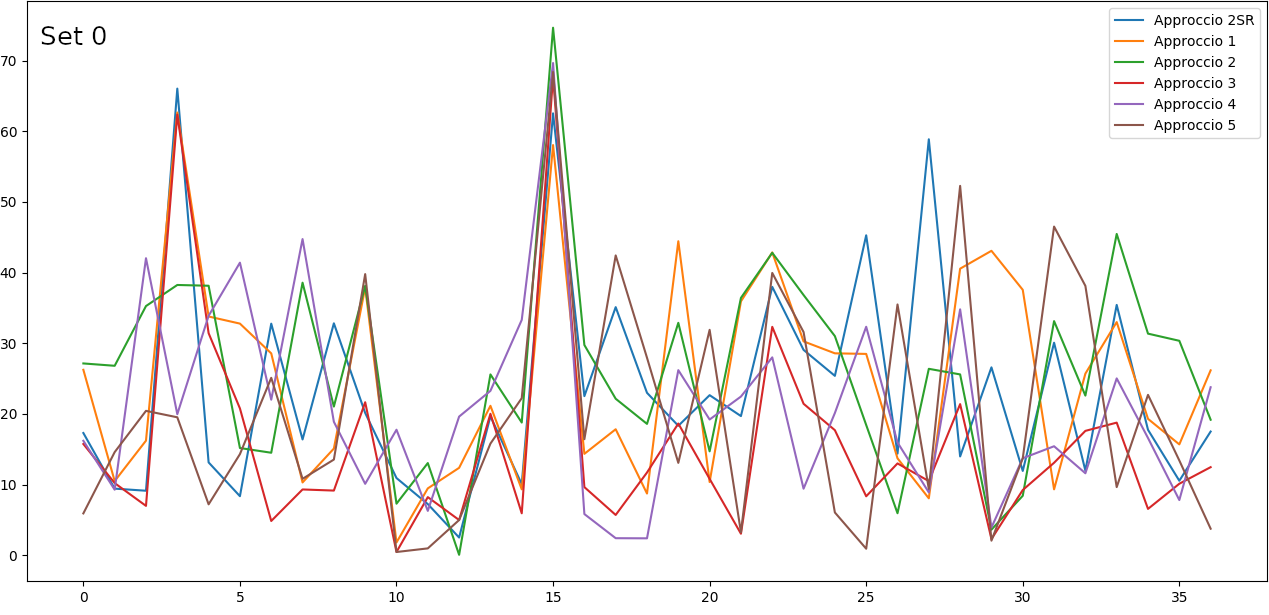
\includegraphics[width=\textwidth]{./Fig/0/all.png}          
        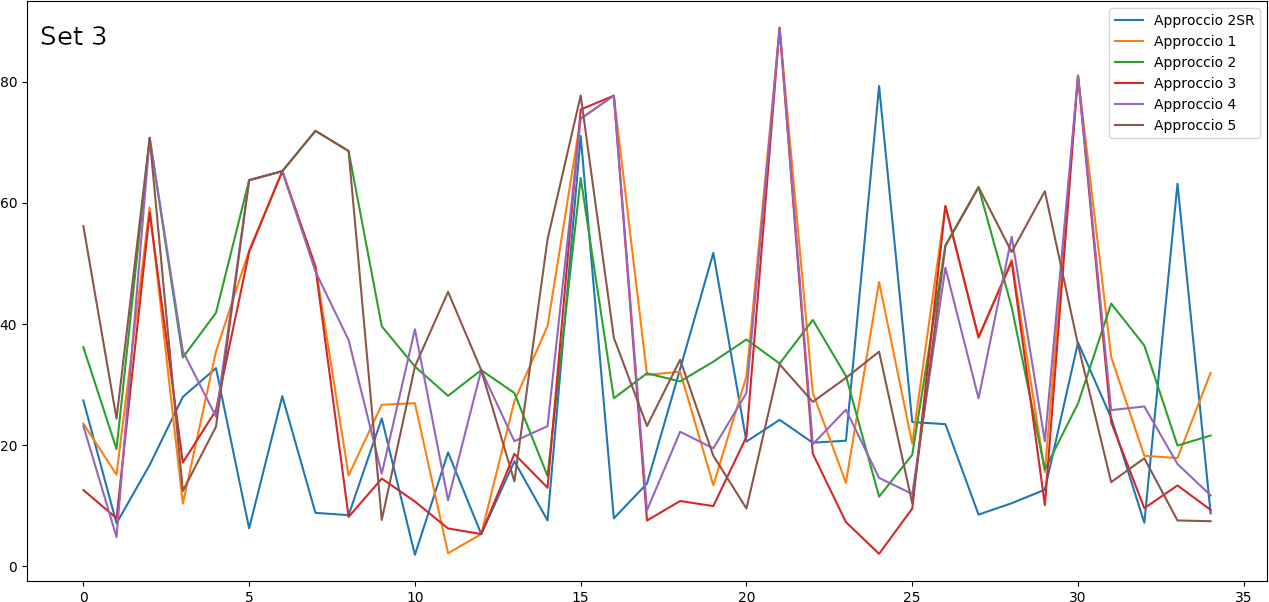
\includegraphics[width=\textwidth]{./Fig/3/all.png}          
      \end{center}
    \end{figure}
\end{document}